\documentclass{article}
\usepackage{fullpage}
\usepackage{amsmath}
\usepackage{amssymb}
\usepackage{graphicx}
\usepackage{url, hyperref}

\renewcommand{\Pr}[1]{\mathbb{P}\left[#1\right]}
\newcommand{\Ex}[1]{\mathbb{E}\left[#1\right]}
\newcommand{\Var}[1]{\text{Var}\left[#1\right]}

\renewcommand{\bf}[1]{\mathbf{#1}}
\newcommand{\bs}[1]{\boldsymbol{#1}}
\newcommand{\mat}[1]{\ensuremath{\begin{pmatrix} #1 \end{pmatrix}}}


\begin{document}

Minqi Xu

20845758

m259xu

\subsection*{Question 1}

\begin{verbatim}
    close all;
    nSamples=10000;
    seed=2;
    rand('seed',seed);
    NSurvive=0;
    rateSurvive=zeros(nSamples,1);

    for n=1:nSamples
        xDist=0;
        for i=1:6
            r=rand(1,1);
            direction=2*pi*r;
            xDist=xDist+cos(direction);
            if(xDist>=4)
                NSurvive=NSurvive+1;
                break;
            end
        end
        rateSurvive(n)=100*NSurvive/n;
    end

    plot(rateSurvive, 'r-', 'linewidth', 2);
    title(sprintf('Rate of neutrons survive (seed=%d)',seed));
    xlabel('Number of neutrons, n');
    ylabel('Rate of neutrons survive (%)');
    axis([1000,10000 0 10]);

    grid on

    pause
    print -dpsc2 volumn.eps
    close
\end{verbatim}

\begin{itemize}
    \item For each neutrons, process a loop for 6 time. Each time randomly 
    select a direction, then move 1 unit length long, and recorded the x-change
    in to xDist, and do a check whether $xDist\geq4$ (if yes, then the neutron survives
    , otherwise, continue the loop until all energy is spent).
\end{itemize}

\begin{figure}
    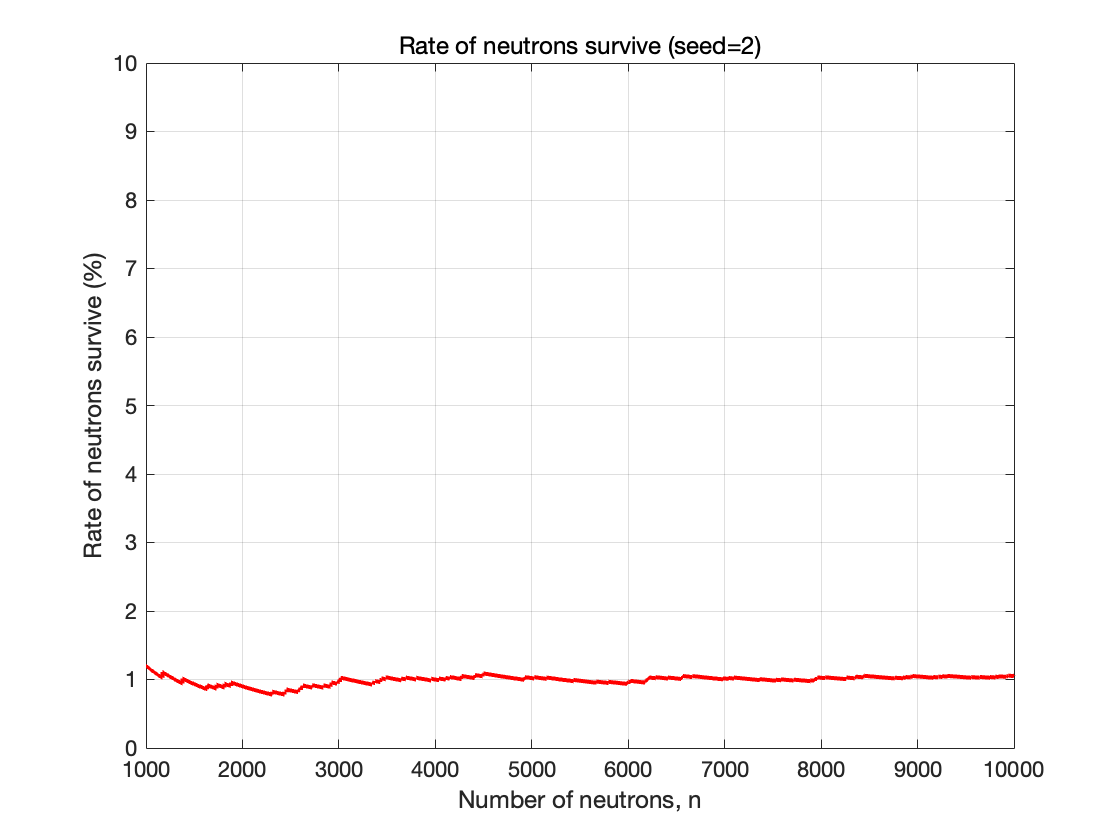
\includegraphics[width=\linewidth]{img/q1.png}
\end{figure}

\newpage

\subsection*{Question 2}
\begin{verbatim}
    close all;
    nSamples=100000;
    seed = 1;
    rand('seed',seed);
    FormFac=zeros(nSamples,1);
    sum=0;

    for n=1:nSamples
        % when sampling points in the right triangle, we can simply sample in
        % the rectangle, for those points out of triangle, we can map it in to
        % the corresponding points in the triangle due to the centrosymmetric
        % to guarantee the sampling is uniform.
        r1=rand(1,1);
        x=2*r1;
        r2=rand(1,1);
        y=r2*(-2)/sqrt(3);
        if(y<(x*(-1)/sqrt(3)))
            % this case the point is out of triangle
           x=2-x;
           y=((-2)/sqrt(3))-y;
        end
        % due to parallel, the two angles in the form factor formula should be
        % the same, for simplicity, we will calculate the cos of it by
        % definition, which is b divided by the distance between random sampled point to
        % origin. Also, visibility term is 1 due to no obstacle.
        dist=sqrt(x^2+y^2+3^2);
        cosepsilon=3/dist;
        sum=sum+(cosepsilon^2/(pi*(dist^2)));
        FormFac(n)=(sum/n)*(2/sqrt(3));
    end

    plot(FormFac, 'r-', 'linewidth', 2);
    title(sprintf('Form Factor (seed=%d)',seed));
    xlabel('Number of points sampled, n');
    ylabel('Form Factor');
    axis([1000,100000 0 0.04]);

    grid on
    pause
    print -dpsc2 FormFac.eps
    close

\end{verbatim}

\begin{itemize}
    \item The method of sampling and getting cosine is mentioned in the comment.
    \item For mapping the out-of-range point to in-range point, the method is do a symmetric
        based on the center of the rectangle (i.e. for old point $(x_{old},y_{old})$, do a symmetric
        based on $(x_c,y_c)$, the result should be $(2x_c-x_{old},2y_c-y_{old})$). Since we are doing
        all things in a same plane (z=3), so z-coordinate is not a problem, it always remains 3 
    \item Also, the result seems converges really fast (about n=300).
\end{itemize}
\begin{figure}
    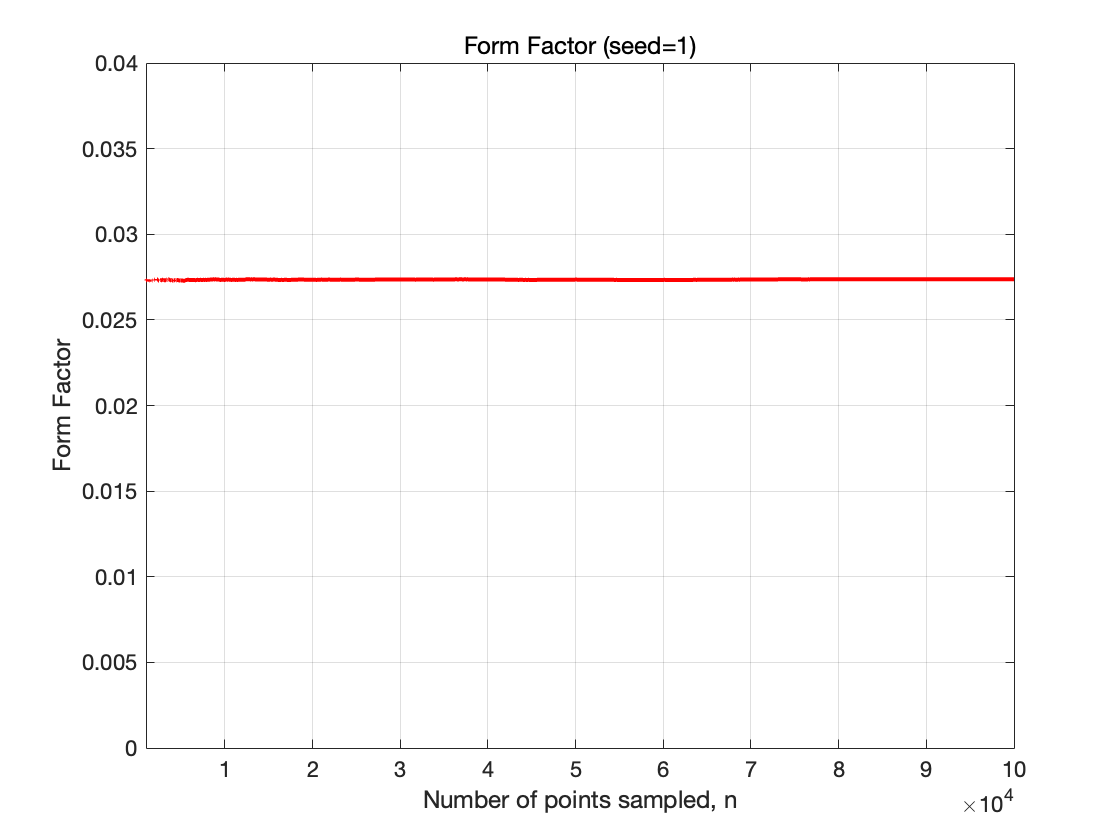
\includegraphics[width=\linewidth]{img/q2.png}
\end{figure}

\newpage
\subsection*{Question 3}
\begin{itemize}
    \item The result obtained in question 2 when n=100000 is 0.0274
    \item For closed form, $F_{dA_i->A_j}=\frac{1}{2\pi} \sum_{i=1}^n \beta_i \cos \alpha_i$, 
    where $\alpha_i$ is the angle subtended by $v_i$, $v_{i+1}$ from origin, and $\beta_i$ is 
    the angle between the plane containing $v_i , v{i+1}$  and origin, and the normal to the differential
    element.
    \item in the specific case of Q2, we have $\cos \alpha_1 = 0, \cos \alpha_3 = 0$
    \item Also, since $\cos \alpha_1 = \cos \alpha_3 = 0, \beta_1$ and $\beta_2$ do not need to be calculated
        for the final answer.
    \item Note that $\beta_2 = arctan(\frac{\frac{2}{\sqrt{3}}}{\sqrt{13}})$
    \item To get $\cos \alpha_2$, first we want the normal vector for plane which contain $v_2, v_3$, and origin
    \item Note that vector (2,0,3) and vector (0,1,0) is in the plane, thus normal vector can be easily get from
        observing, thus the normal vector is (-3,0,2)
    \item Next, we have $\cos \alpha_2 = \frac{\vec{n_1} \cdot \vec{n_2}}{|\vec{n_1}||\vec{n_2}|} = \frac{2}{\sqrt{13}}$
    \item Finally, substitue all values in to the formula we get $F=0.0273621155$
    \item Relative error of my result is $\frac{0.0274-0.0273621155}{0.0273621155} \approx 0.1385\%$
    \item Reference for this question: 
    \item Stark, Michael M. and Richard F. Riesenfeld. “Exact Radiosity Reconstruction and Shadow Computation Using Vertex Tracing.” (1999).
    \item Cohen, Michael F. and John R. Wallace. “Radiosity and realistic image synthesis.” (2016) pp.70.
  

\end{itemize}

\newpage
\subsection*{Question 4}
\begin{itemize}
    \item According to $L_i=\frac{\rho_i}{\pi} \frac{\Phi_i}{A_i}$
    \item the value of radiance of triangle should be $\frac{0.25}{\pi} \frac{0.0274\times 100W}{0.5\times 2\times \frac{2}{\sqrt{3}}}\approx 0.1888 \frac{W}{m^2sr}\approx 0.19 \frac{W}{m^2sr}$
\end{itemize}

\newpage
\subsection*{Question 5}
\begin{align}
    \int_0^{2\pi} \int_0^R k(1-\frac{r}{R})drd\theta & = k\cdot \int_0^{2\pi} \int_0^R (1-\frac{r}{R})drd\theta\\
    & = k\cdot \int_0^{2\pi} \lbrack r - \frac{r^2}{2R}\rbrack ^R_0 d\theta\\
    & = k\cdot \int_0^{2\pi} \frac{R}{2} d\theta\\
    & = \pi kR = 1 \implies k = \frac{1}{\pi R}\\
    \int_0^{2\pi} \int_0^{\frac{R}{2}} k(1-\frac{r}{R})drd\theta & = k\cdot \int_0^{2\pi} \int_0^{\frac{R}{2}} (1-\frac{r}{R})drd\theta\\
    & = k\cdot \int_0^{2\pi} \lbrack r - \frac{r^2}{2R}\rbrack ^{\frac{R}{2}}_0 d\theta\\
    & = k\cdot \int_0^{2\pi} \frac{3R}{8} d\theta\\
    & = k\cdot \frac{3}{4}R\pi = \frac{3}{4} = 0.75
\end{align}

\newpage
\subsection*{Bonus Question}
\begin{align}
    \int_0^{\phi} \int_0^{\theta} \frac{1}{4\pi} (\frac{1-g^2}{(1+g^2-2gcos\theta)^{\frac{3}{2}}}) d\theta d\phi\\
    \int_0^{\phi} \frac{1}{2\pi} d\phi &= \frac{\phi}{2\pi}\\
    &= \xi_2 \implies \phi=2\pi \xi_2\\
    \int_0^{\theta} \frac{1}{2} \frac{1-g^2}{(1+g^2-2gcos\theta)^{\frac{3}{2}}} d\theta
\end{align}

\end{document}
